
\begin{frame}{‌جستجوی سطح‌اول}
\begin{itemize}\itemr
\item[-]
جستجوی سطح‌اول
\fn{1}{breadth-first search}
یکی از ساده‌ترین الگوریتم‌های جستجوی گراف است که در بسیاری از الگوریتم‌های گراف استفاده می‌شود. برای مثال الگوریتم دایکسترا برای یافتن کوتاهترین مسیر بین دو رأس از جستجوی سطح‌اول استفاده می‌کند.
\item[-]
به ازای گراف دلخواه
\m{G=(V,E)}
و یک رأس مبدأ
\fn{2}{source vertic}
به نام
\m{s}
، الگوریتم جستجوی سطح‌اول همهٔ یال‌های گراف
\m{G}
را با شروع از رأس
\m{s}
بررسی می‌کند.
\item[-]
با شروع از رأس
\m{s}
، الگوریتم سطح‌اول ابتدا رئوسی را بررسی می‌کند که به
\m{s}
نزدیک‌ترند،
بدین معنی که برای رسیدن به آن رئوس از
\m{s}
باید از تعداد یال‌های کمتری عبور کرد.
\end{itemize}
\end{frame}


\begin{frame}{‌جستجوی سطح‌اول}
\begin{itemize}\itemr
\item[-]
یال‌هایی که در جستجوی سطح‌اول به ترتیب بررسی می‌شوند، یک درخت سطح‌اول می‌سازد که ریشهٔ آن
\m{s}
است و به ازای هر یک از رئوس
\m{v}
، یک مسیر ساده از
\m{s}
به
\m{v}
کوتاهترین مسیر از
\m{s}
به
\m{v}
در گراف را نشان می‌دهد.
در اینجا کوتاهترین مسیر درواقع مسیری است که دارای کمترین تعداد یال باشد.
\item[-]
جستجوی سطح‌اول، بدین دلیل سطح‌اول نامیده می‌شود که به ازای هر رأس
\m{v}
ابتدا رئوس مجاور آن بررسی  می‌شوند، قبل از اینکه رئوس مجاور مجاور آن بررسی شوند.
بنابراین اگر نزدیکترین رئوس به یک رأس را در سطح در نظر بگیریم و دورترین رئوس را در عمق، جستجوی سطح‌اول، قبل از بررسی رئوس در عمق، همهٔ رئوس در سطح را بررسی می‌کند.
بنابراین برخلاف جستجوی عمق اول که به ازای هر رأس
\m{v}
یک رأس مجاور مجاور
\m{v}
 ممکن است قبل از یک رأس مجاور
\m{v}
  پیمایش شود، در جستجوی سطح‌اول همهٔ رئوس مجاور
\m{v}
قبل از پیمایش رئوس مجاور مجاور 
\m{v}
پیمایش می‌شوند.
\end{itemize}
\end{frame}


\begin{frame}{‌جستجوی سطح‌اول}
\begin{itemize}\itemr
\item[-]
 در جستجوی سطح‌اول با شروع از رأس
\m{s}
ابتدا رئوس مجاور
\fn{1}{adjacent}
 یا همسایه‌هایی
\fn{2}{neighbour}
  بررسی می‌شوند که فاصلهٔ آنها از
\m{s}
برابر ۱ است، سپس همسایه‌ها با فاصلهٔ ۲ بررسی می‌شوند، پس از آن همسایه‌ها با فاصلهٔ ۳ و به همین ترتیب الی آخر، تا وقتی که همه رئوس بررسی شده باشند.
\item[-]
در جستجوی سطح‌اول از یک صف استفاده می‌شود که در آن ابتدا همسایه‌ها با فاصله ۱، سپس همسایه‌ها با فاصلهٔ ۲ و به همین ترتیب الی آخر در صف قرار می‌گیرند. بنابراین با خارج کردن همسایه‌ها از صف به ترتیب فاصله، گراف به صورت سطح‌اول بررسی می‌شود.
\end{itemize}
\end{frame}


\begin{frame}{‌جستجوی سطح‌اول}
\begin{itemize}\itemr
\item[-]
در الگوریتم جستجوی سطح‌اول می‌توانیم برای هر رأس ۳ رنگ در نظر بگیریم : سفید، خاکستری و سیاه. همهٔ رئوس در ابتدا به رنگ سفید هستند و رئوسی که هیچ مسیری از
\m{s}
به آنها وجود ندارد تا انتها به رنگ سفید باقی می‌‌مانند. وقتی یک رأس برای اولین بار با شروع از
\m{s}
پیمایش می‌شود، آن رأس به رنگ خاکستری تبدیل می‌شود. رنگ خاکستری بدین معنی است که آن رأس در مرز جستجو قرار گرفته است. مرز جستجو در واقع مرز میان رئوس پیمایش نشده و رئوس پیمایش شده است. صفی که در جستجوی سطح‌اول استفاده می‌شود، شامل همهٔ رئوس خاکستری است.
\item[-]
رئوس خاکستری به ترتیب از صف خارج می‌شوند و به رنگ سیاه تبدیل می‌شوند و رئوس سفید همسایهٔ آنها که تاکنون پیمایش نشده‌اند به رنگ خاکستری تبدیل می‌شوند و وارد صف می‌شوند.
\end{itemize}
\end{frame}


\begin{frame}{‌جستجوی سطح‌اول}
\begin{itemize}\itemr
\item[-]
یک الگوریتم جستجوی سطح‌اول، یک درخت سطح‌اول می‌سازد که ریشهٔ آن رأس
\m{s}
است. هرگاه در فرایند جستجو، یک رأس سفید
\m{v}
که در لیست همسایه‌های رأس خاکستری
\m{u}
 قرار دارد پیدا می‌شود، رأس
\m{v}
و یال
\m{(u,v)}
به درخت اضافه می‌شوند. می‌گوییم رأس
\m{u}
، سَلَف
\fn{1}{predecessor}
یا پدر رأس
\m{v}
و رأس
\m{v}
خَلَف
\fn{2}{successor}
یا فرزند رأس
\m{u}
در درخت سطح‌اول است. از آنجایی که هر رأس قابل دسترس از طریق
\m{s}
تنها یک بار بررسی می‌شود، هر رأس تنها یک پدر دارد.
\item[-]
تنها رأس ریشه، یعنی رأس
\m{s}
  دارای پدر نیست.
\item[-]
اگر رأس
\m{u}
بر روی یک مسیر ساده درخت از ریشه
\m{s}
به رأس
\m{v}
قرار بگیرد، آنگاه رأس
\m{u}
جد
\fn{3}{ancestor}
رأس
\m{v}
است و رأس
\m{v}
نوادهٔ
\fn{4}{descendant}
رأس
\m{u}
است.
\end{itemize}
\end{frame}


\begin{frame}{‌جستجوی سطح‌اول}
\begin{itemize}\itemr
\item[-]
در الگوریتم جستجوی سطح‌اول که بررسی خواهیم کرد،
\code{v.color}
رنگ رأس
\m{v}
است که می‌تواند سفید، خاکستری یا سیاه باشد،
\code{v.d}
فاصلهٔ رأس
\m{v}
از رأس
\m{s}
است و
\code{v.pred}
پدر رأس
\m{v}
است.
\item[-]
 رأس
\code{v.pred}
پدر
\fn{1}{predecessor}
 رأس
\code{v}
است، و رأس
\code{v}
فرزند
\fn{2}{successor}
رأس
\code{v.pred}
.
\end{itemize}
\end{frame}


\begin{frame}{‌جستجوی سطح‌اول}
\begin{itemize}\itemr
\item[-]
الگوریتم زیر جستجوی سطح‌اول را نشان می‌دهد.
\begin{algorithm}[H]\alglr
  \caption{Breadth-First Search} 
  \begin{algorithmic}[1]
   \Func{BFS}{G,s}
   \For{each vertex u $\in$ G.V - \{s\} }
   			\State u.color = White
   			\State u.d = $\infty$
   			\State u.pred = Nil
   	\EndFor
   	\State s.color = Gray
   	\State s.d = 0
   	\State s.pred = Nil
   	\State Q = $\emptyset$
   	\State Enqueue(Q,s)         
  \end{algorithmic}
  \label{alg:merge}
\end{algorithm}
\end{itemize}
\end{frame}


\begin{frame}{‌جستجوی سطح‌اول}
\begin{algorithm}[H]\alglr
  \caption{Breadth-First Search} 
  \begin{algorithmic}[1]
  \setcounter{ALG@line}{9}
   %\Func{Bfs}{G,s}			%\LeftComment{}
        \While{!empty(Q)}
        		\State u = Dequeue(Q)
        		\For{each vertex v in G.Adj[u]}		\LeftComment{search the neighbors of u}
        			\If{v.color == White}		\LeftComment{is v being discovered now?}
        				\State v.color = Gray
        				\State v.d = u.d + 1
        				\State v.pred = u
        				\State Enqueue(Q,v)		\LeftComment{v is now on the frontier}
        			\EndIf
        		\EndFor
        		\State u.color = Black		\LeftComment{u is now behind the frontier}
        \EndWhile		                   
  \end{algorithmic}
  \label{alg:merge}
\end{algorithm}
\end{frame}


\begin{frame}{‌جستجوی سطح‌اول}
\begin{itemize}\itemr
\item[-]
در شکل زیر یک گراف به صورت سطح‌اول پیمایش شده است.
\begin{figure}
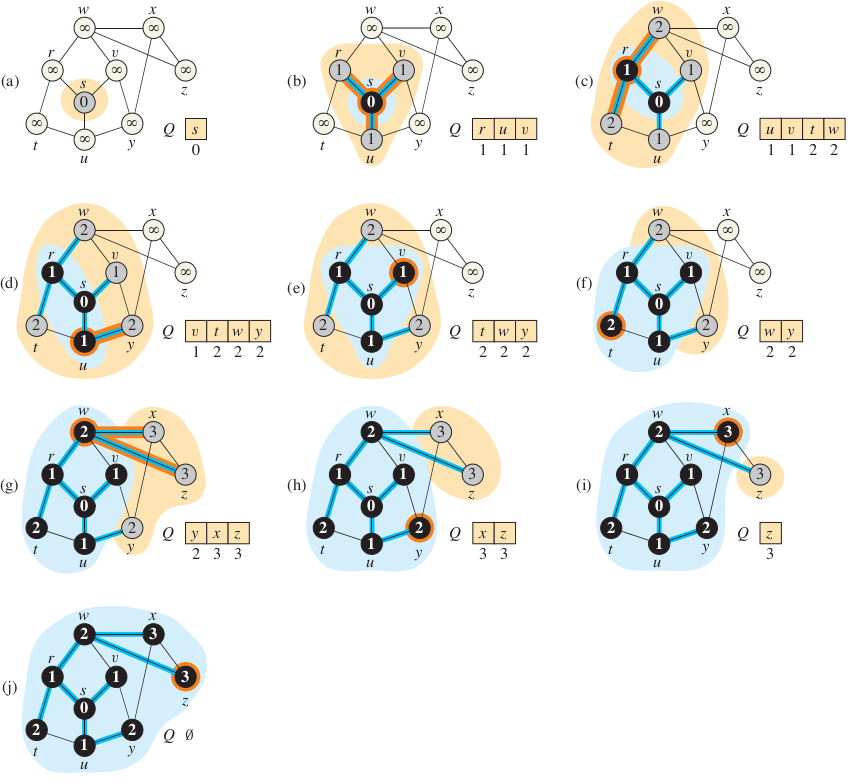
\includegraphics[width=0.5\textwidth]{figs/chap07/557-bfs}
\end{figure}
\end{itemize}
\end{frame}


\begin{frame}{‌جستجوی سطح‌اول}
\begin{itemize}\itemr
\item[-]
تحلیل الگوریتم جستجوی سطح‌اول : برای تحلیل الگوریتم جستجوی سطح‌اول می‌توانیم از تحلیل تجمعی استفاده کنیم. در این الگوریتم هیچ‌گاه یک رأس از رنگ خاکستری یا سیاه به رنگ سفید در نمی‌آید. هر رأس حداکثر یک بار وارد صف می‌شود و بنابراین هر رأس حداکثر یک بار از صف خارج می‌شود. عملیات اضافه کردن و برداشتن از صف در زمان
\m{O(1)}
انجام می‌شود.
خارج کردن رئوس از صف در زمان
\m{O(V)}
انجام می‌گیرد.
همچنین بررسی لیست مجاورت هر رأس حداکثر یک‌بار انجام می‌شود و مجموع طول همهٔ لیست‌های مجاورت برابر است با
\ath{E}
، بنابراین زمان لازم برای اجرای الگوریتم برابراست با
\m{O(V+E)}~.
نتیجه می‌گیریم جستجوی سطح‌اول در زمان خطی نسبت به اندازه لیست مجاورت اجرا می‌شود.
\item[-]
می‌توان ثابت کرد الگوریتم جستجوی سطح‌اول کوتاهترین مسیر از
\m{s}
به هریک از رئوس را محاسبه می‌کند.
\end{itemize}
\end{frame}

\iffalse
\begin{frame}{‌جستجوی سطح‌اول}
\begin{itemize}\itemr
\item[-]
حال می‌خواهیم اثبات کنیم الگوریتم جستجوی سطح‌اول کوتاهترین مسیر از رأس مبدأ
\m{s}
به هریک از رئوس گراف را پیدا می‌کند. فاصله کوتاهترین مسیر
\fn{1}{shortest path distance}
\m{\delta(s,v)}
از رأس
\m{s}
به
\m{v}
کمترین تعداد یال‌هایی است که در یک مسیر از
\m{s}
به
\m{v}
می‌توان پیمود. اگر هیچ مسیری از
\m{s}
به
\m{v}
وجود نداشته باشد، آنگاه
\m{\delta(s,v) = \infty}
مسیری که طول آن
\m{\delta(s,v)}
باشد کوتاهترین مسیر
\fn{2}{shortest path}
از
\m{s}
به
\m{v}
است.
\end{itemize}
\end{frame}
\fi